\chapter{实验一:眼动实验}
\label{exp1}

\section{研究目的}
眼动实验的研究对象是审美主体,即人。根据流畅理论,正面的审美反馈往往意味着更为流畅的眼动行为。通过眼动仪对被试者眼动行为记录得到的数据,探讨眼动行为与美感的关系,并试图论证以下假设:

\begin{enumerate}
  \item 正面审美反馈所对应的眼动行为在整体上具有在面对多个视觉注意线索时,更少冲突地作出选择的特点
  \item 正面审美反馈所对应的眼动行为在局部上具有面对一个视觉重点时更聚焦地趋向一个兴趣点的特点。
\end{enumerate}

\section{实验与数据}
我们的实验模拟视觉自然而突然地降落到网页页面上。唯一不自然的部分是被我们称为“限时曝光”的形式,这种方式将强制被试对页面进行快速而全面的视觉探索而不是具体而局部的信息收集。在三张用于适应性缓冲的网页过后,被试者将意识到他们只有几秒钟的时间来看每一张展示的页面。这样的设计的合理性在于,正如我们所已经知道的,为了避免在糟糕的页面上的无意义停留,用户习惯于在到达一个新的页面的几秒钟内作出去留的决定。

对于研究早期的无意识的注视行为而言,几秒钟的限时曝光就已足够。同时,这种方式避免了因被试者的视觉疲劳而造成的误差

\subsection{设备}
实验使用的眼动设备是Tobii的T-50眼动仪和配套的Tobii Studio软件。该眼动仪的屏幕分辨率是$1280\times1024px$。

\subsection{实验样本}
实验采用对40张网页页面的截图作为测试的样本。为了让这些页面对好/坏的美感更具有代表性,我们通过一个评选最好看的网页设计的网站(the best designs\footnotemark[1])和一个评选最丑的网页设计的网站( websites from hell\footnotemark[2])两个网站来分别采集好的页面样本和坏的页面样本。只采集了这两个网站上的基数页面。

\footnotetext[1]{
the best design:
\href{https://www.thebestdesigns.com}{https://www.thebestdesigns.com}
}

\footnotetext[2]{
websites from hell:
\href{https://websitesfromhell.net}{https://websitesfromhell.net}
}

包含广为人知的图标或人脸以及包含非拉丁字符的页面被筛除以避免来自非美学的社会因素的干扰。最终我们从上述两个网站个筛选出20个网页,并在$1280\times800$的分辨率下对他们进行截图以匹配我们使用的眼动仪的分辨率。截图包含了网页浏览器的窗口。图\ref{fig:all}展示了实验用到的所有的样本页面。

\begin{figure*}
  \centering
  \includegraphics[width=0.85\textwidth]{fig/fig_all.jpg}
  \caption{所有在眼动实验中被用到的图片。按照美感评分的高低从上至下,从左至右地排列}
  \label{fig:all}
\end{figure*}

\subsection{被试者}
一共30名被试者(13男,17女)参与了眼动实验。他们都是来自上海交通大学不同院系的学生。除去一些学生来自韩国的学生,其余的学生都来自中国。他们的年龄段在19到27岁之间。

\subsection{实验环境}
实验在一个安静的房间内进行。房间的窗帘被拉上考虑到不可控的自然光源可能造成屏幕反光。眼动仪被放置在一面纯白色的墙壁前以避免可能的注意力分散。

\subsection{实验过程}
每名被试被要求以平时闲逛网页的状态来浏览被试的网页样本。被试身体略微前倾地坐在一张办公椅上,放置他或她的下巴到一个高而柔软的支撑物上并调整位置以使实现距眼动仪的屏幕60厘米。被试的手肘自然放置在,一首握着鼠标,虽然该鼠标的动作不会带来交互行为。

为了减少疲劳,实验被分成时隔一分钟休息的两阶段进行。每阶段眼动仪随机展示所有40张样本页面中的一半。每张页面只展示3秒钟,紧接着是一个1秒钟的黑屏作为缓冲。每个阶段最开始都会展示三张不参与实验的假页面作为缓冲,以使被试适应实验的节奏。被试在整个实验过程中不会受到任何的提示和干扰。

对实验样本页面的主观评分被安排在所有眼动实验结束之后,与之分离。在评分过程中,被试将再次无时限地浏览每一张样本网页,通过“好”和“坏”两个选项来评价每一张页面美感体验。

所有的被试都确认他们从未见过任何一张实验样本页面。

\subsection{数据采集}
实验结束后,每张样本页面都根据其获得的“好评”的比例获得一个介于0-1之间的美感得分。图\ref{fig:score}展示了所有40张样本页面在美感得分上的频率分布直方图。

评分结果显然呈现出了二值化的特征。20张评分低于0.5的页面和来自\href{https://websitesfromhell.net/}{websites from hell}的页面完全重合。即从美感角度而言,这些页面是毫无疑问的“坏”页面。

眼动数据方面,T50眼动仪通过一个固定的50Hz的频率采集被试眼睛的聚焦位置。通过差值算法获得连续的眼动速度,然后通过阈值来确定眼动注视在哪段时间内发生(眼动速度几乎等于0的时段)。

通过眼动仪获得的原始数据是有一系列的注视构成的。每个注视包含了四个参数信息:开始时间、持续时长、在屏幕上的横纵坐标位置。后续我们将基于这种形式的原始眼动数据展开分析。

\begin{figure}[H]
  \centering
  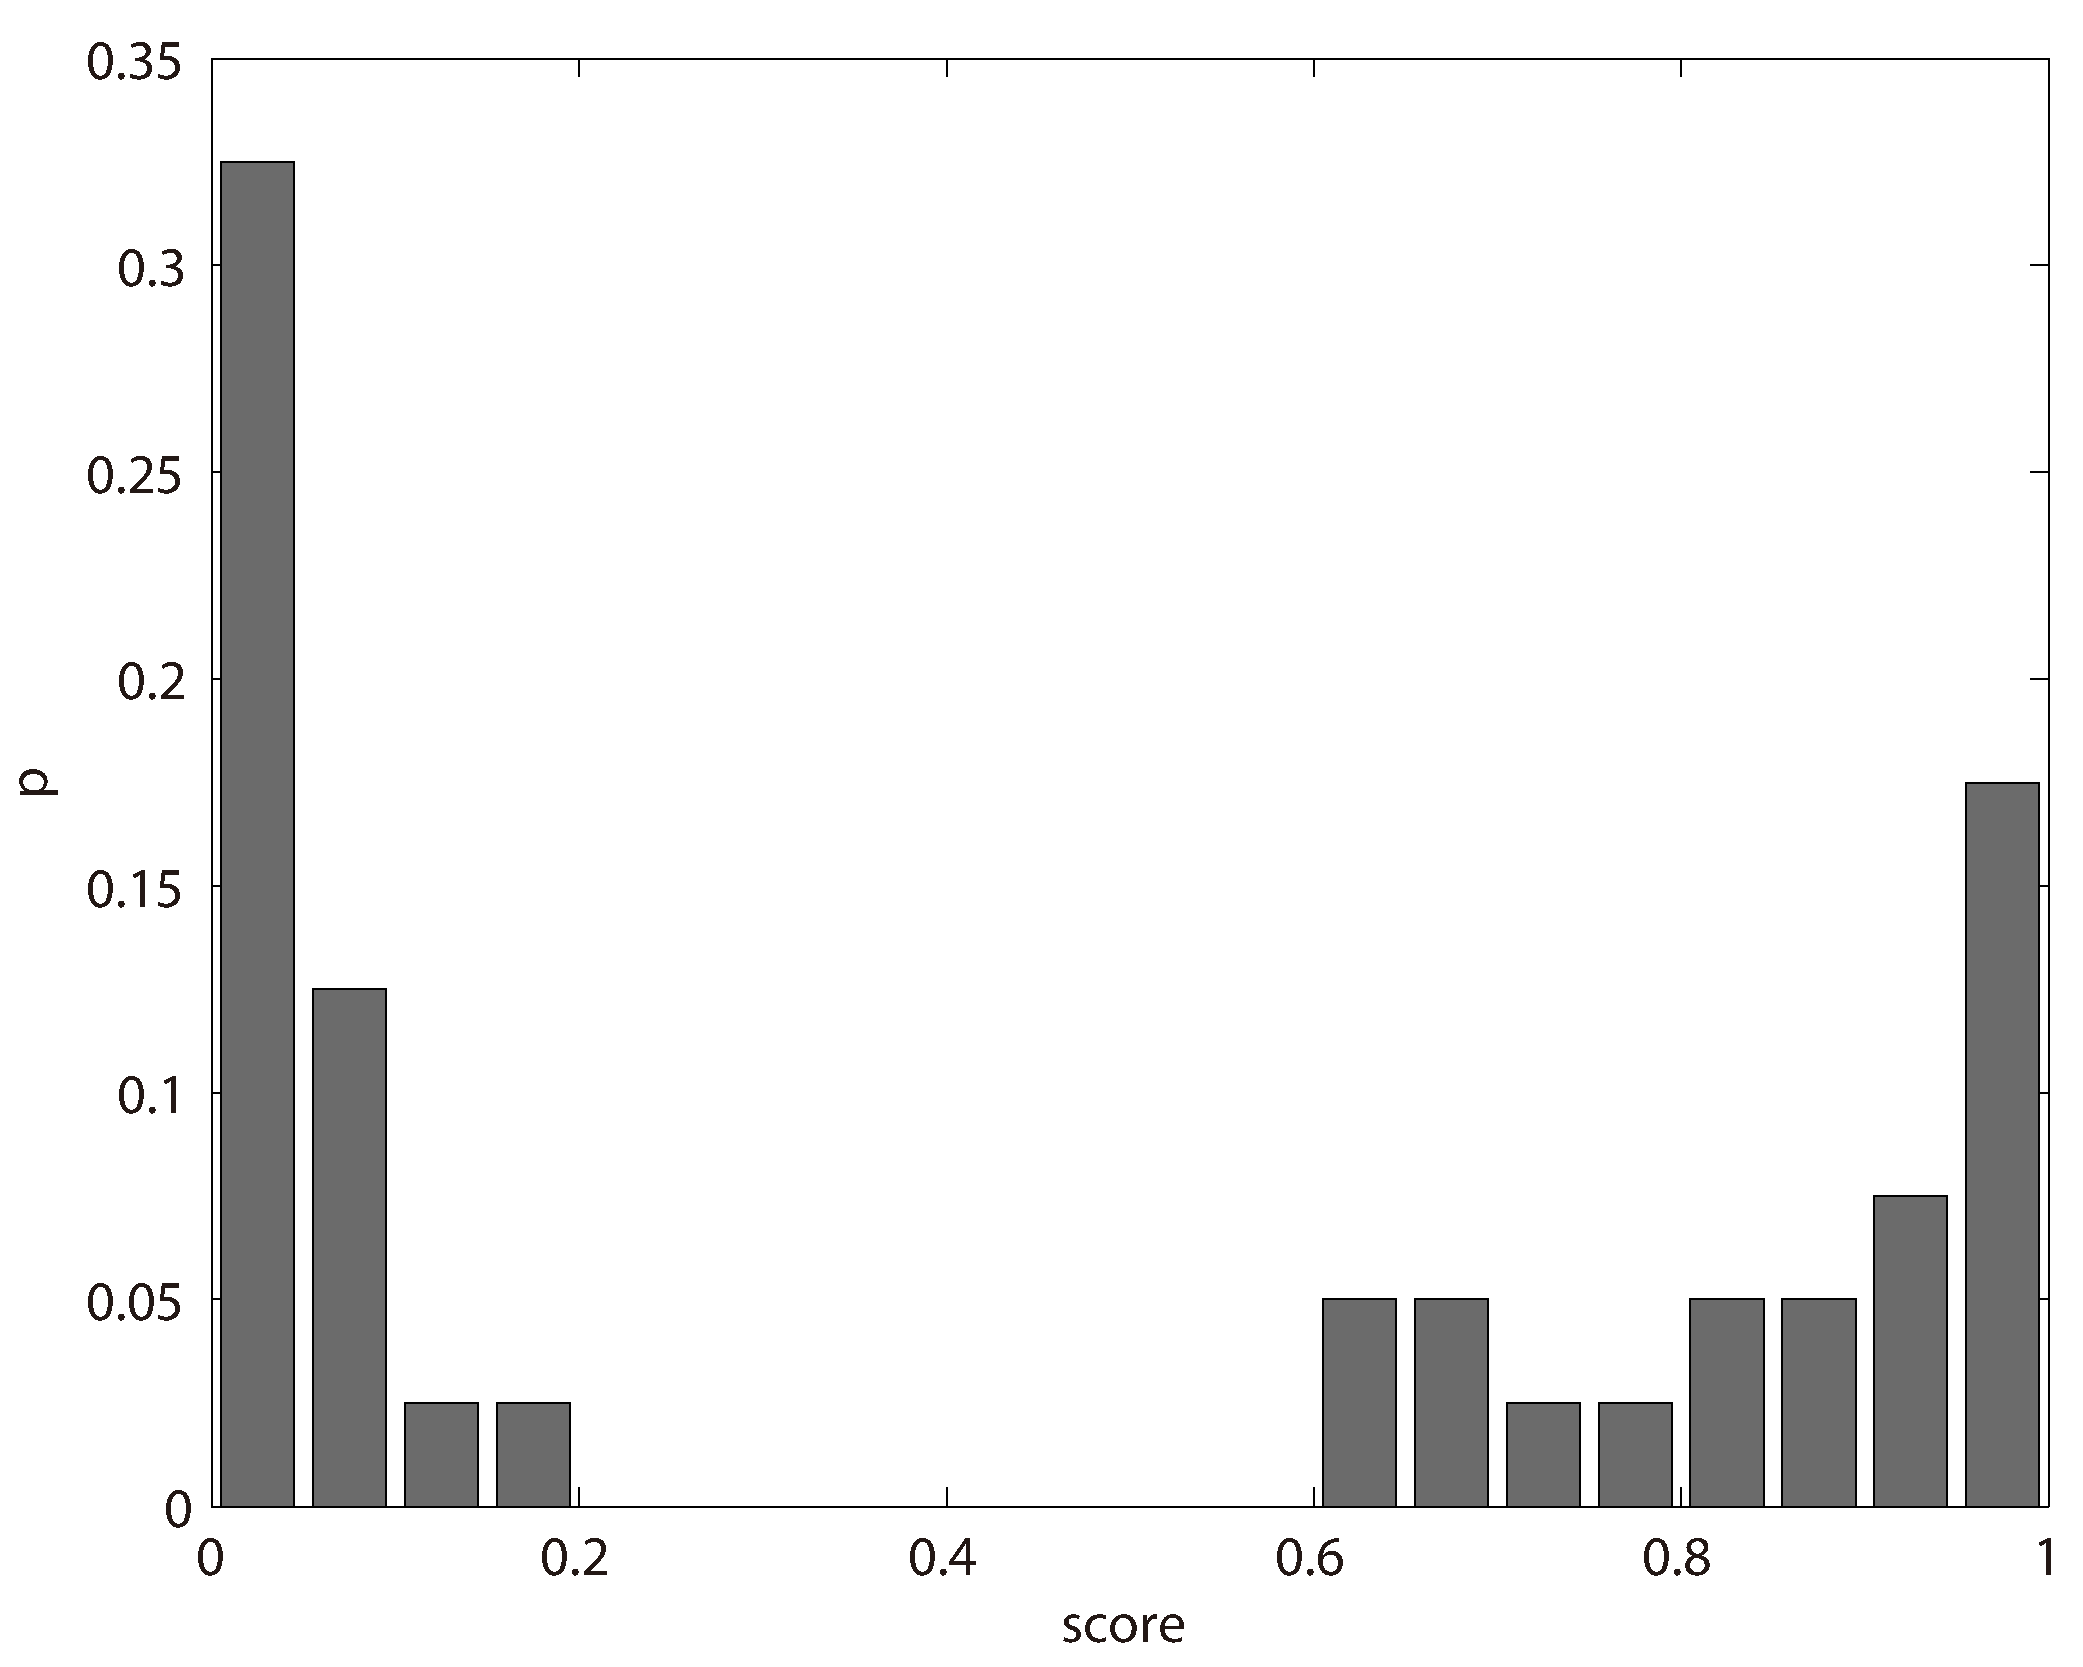
\includegraphics [width=0.7\textwidth]{fig/fig_score.pdf}
  \caption{实验页面的评分的频率分布直方图。可以看到好坏美感的评分被清晰地二值化分开成了两个具有好坏页面代表性的组别。差的网页的评分的一致性相比好的网页更高,一定程度上证实了人们往往对对象的不美观上更容易达成一致【】}
  \label{fig:score}
\end{figure}



\section{分析}
\label{sec:exp1-ana}

\subsection{传统的眼动指标}
首先,对我收集到的眼动数据,我们试验一些传统的描述性指标。这些指标大部分都在第\ref{chap:related}章相关研究中被提及:

\begin{itemize}
  \item 注视总数
  \item 平均注视时长
  \item 注视时长的标准差
  \item 平均扫视距离
  \item 扫视距离的标准差
  \item AOI个数
  \item AOI中注视的平均个数
  \item AOI中注视个数的标准差
\end{itemize}

上面提到的AOI是Area of interests的缩写,表示视觉兴趣点,是通过对页面上捕捉到的所有注视进行空间聚类得到空间区块。我们采用Tobii Studio软件包中自带的默认AOI聚类算法来获得这些AOI区块。图\ref{fig:aoi}以参与实验的一张样本页面为例,标出了它的AOI聚类情况。

\begin{figure}[H]
  \centering
  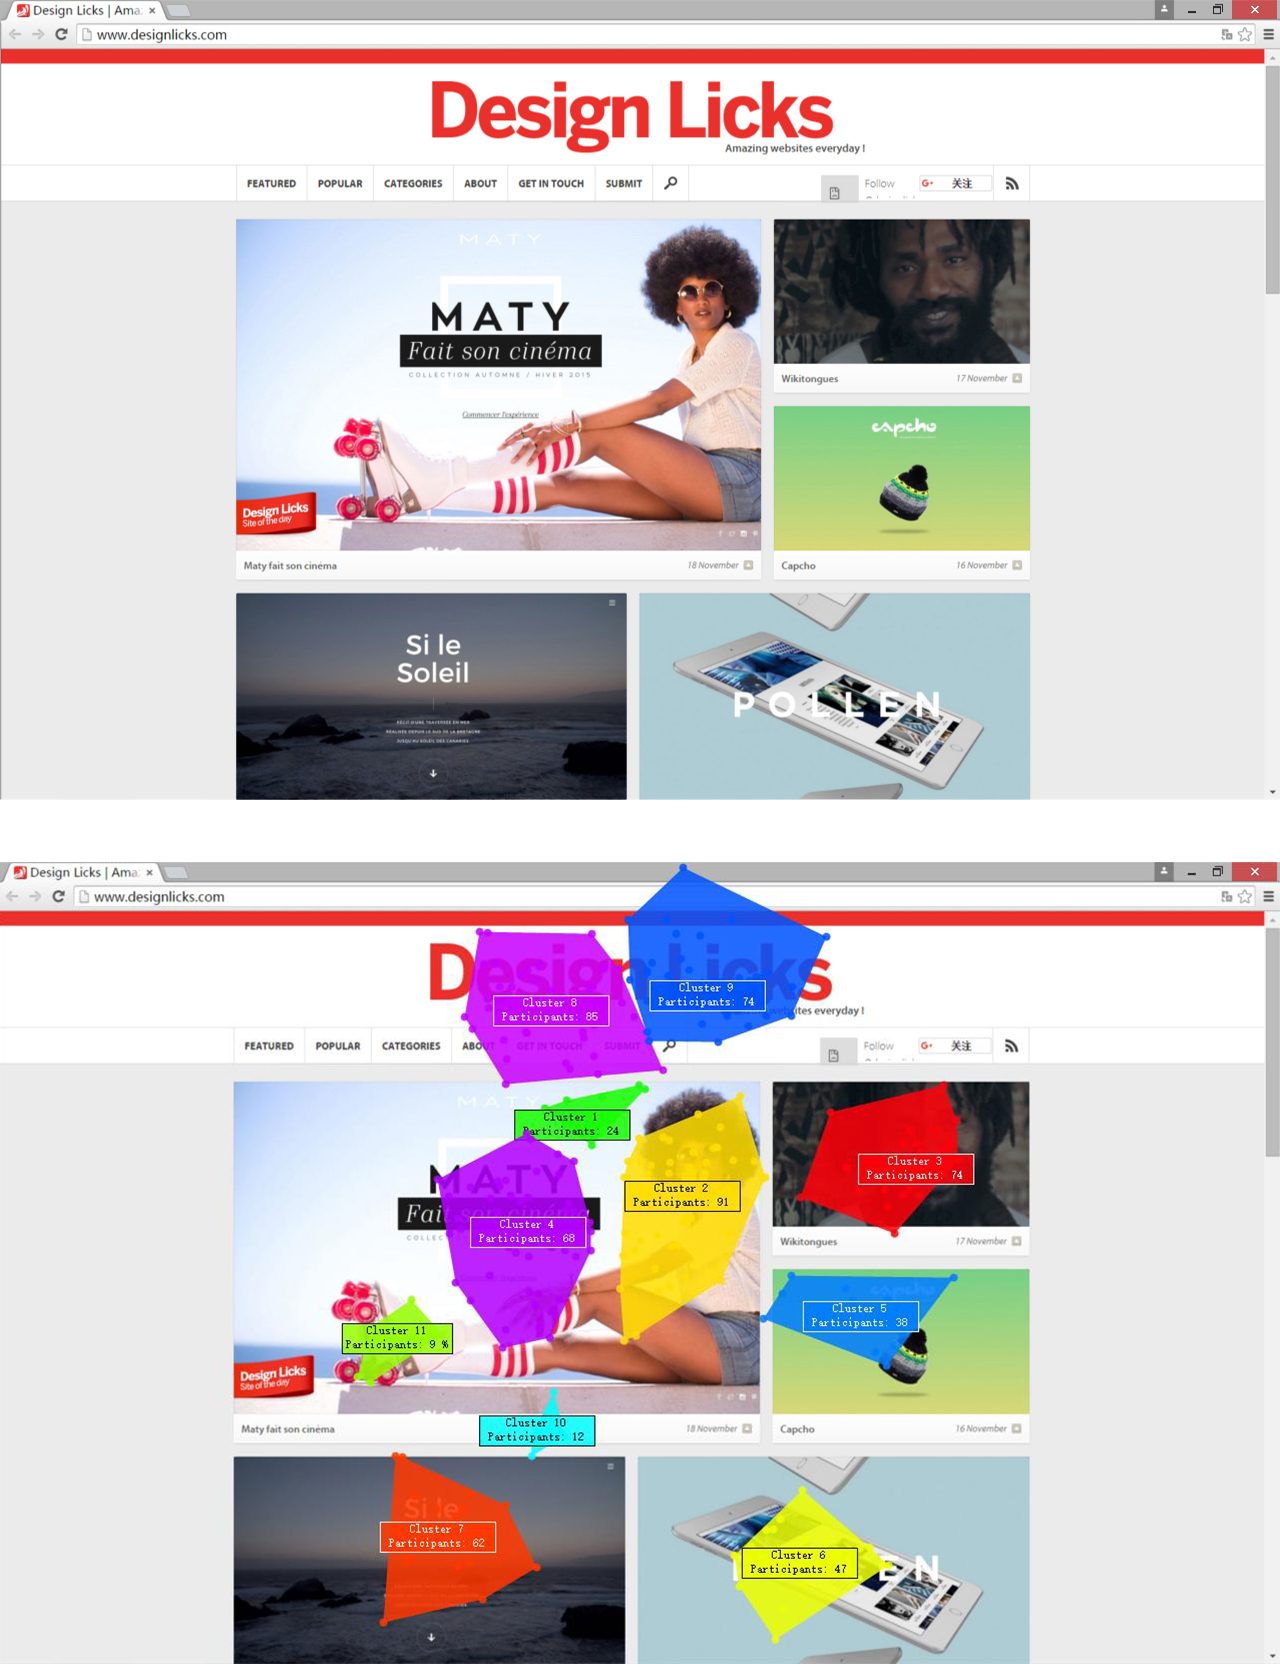
\includegraphics [width=0.85\columnwidth]{fig/fig_AOI.jpg}
  \caption{AOI聚类的示意图。上方是参与眼动实验的一张页面,下方是该页面与其AOI聚类结果的重叠图。AOI聚类通过Tobii Studio软件自带的聚类算法来实现。该页面一共产生了11个AOI聚类区块。}
  \label{fig:aoi}
\end{figure}

表格\ref{tab:traditional}列出了参与计算的所有传统指标在与美感评分的关联性方面的表现,包括每个指标与评分的线性相关系数和对好坏页面组别进行方差分析的p值。在0.05的置信系数上,只有注视个数通过了方差检验($p=0.04$)。注视个数表现出了微弱的与美感评分的正相关性,也即在相同的曝光时间内,好看的页面普遍获得了更多的眼动注视,拥有更活跃的眼动反馈。

\begin{table}[H]
  \centering
  \begin{tabular}{lrr}
    \hline
     &相关系数 & 方差显著性 \\
    \hline
    注视总数 & 0.3322 & 0.0429 \\
    平均注视时长 & -0.1526 & 0.3227 \\
    注视时长的标准差 & 0.1165 & 0.6219 \\
    平均扫视距离 & -0.2203 & 0.0871 \\
    扫视距离的标准差 & -0.1933 & 0.2732 \\
    AOI个数 & -0.2607 & 0.1631 \\
    AOI中注视的平均个数 & 0.3228 & 0.0782 \\
    AOI中注视个数的标准差 & 0.2556 & 0.0991 \\
    \hline
  \end{tabular}
  \caption{传统的眼动指标与美感关联性的表现。这些指标都直接提取自注视、扫视和AOI聚类这些常见的眼动度量,只有注视的总数表现出了微弱的方差检验显著性。}
  \label{tab:traditional}
\end{table}


\subsection{眼动过程中的熵}
熵在信息论和热力学中都有定义。概念上,它用来表达一个系统的混乱度、无序程度,或者反过来说对有序性、确定性的缺乏。

本研究中的视觉熵的概念是基于香农的信息熵理论的。信息熵是基于概率空间的一种对不确定性的度量。对一个具有离散的概率空间$\{x_1, ..., x_n\}$和分布$P(X)$和的随机变量$X$,信息熵$H$(希腊大写字母Eta)定义为:

$$H(X)~=~-\sum_{i=1}^n P(x_i)\cdot log_{2}P(x_i)$$

$H(X)$越大,分布$P(x_i)$就更混乱度而不确定,反之则更有更小的不确定性。

接下来我们借助信息熵来分析眼动两个维度:眼动在AOI间的跳转和注视在空间上的分布。

\subsubsection{注视转移中的熵}
最早在Tole et al【】的关于认知负担的研究中把熵的概念引入到眼动数据的分析中。他用熵来描述11名飞行员在执行不同任务时观察行为的变化。该模型在之后也被应用在一项关于驾车时的眼动行为的研究中。【】
Hooge【】使用一种类似的称之为“视觉路径熵”(scan path entropy)的概念来度量对一个特定视觉兴趣点的眼动一致性。

下面我们依照Tole的基于马尔科夫链的视觉熵的定义,分析其与美感评分的关联性。

这种熵描述了眼镜在注视之间转移的确定性。在实验中,注视的位置的概率空间的大小是$1024\times800$,等同于屏幕的分辨率。如此庞大的概率空间使得不同被试之间的眼动序列无法进行比较。对此,Tole的做法是把整个视觉范围人为分割为一些的区域。在本实验中,我们借助系统自动聚类生成的AOI来完成这种区块划分,并考察眼睛在这些AOI间的跳转。跳转是由视觉注意机制所驱动的,在无意识的情况下从当前的目标切换到外围视觉的目标【】,这也就是Berlyne所提出的全面视觉探索的意思。通过AOI对注视的聚类,我们可以将来自原始数据的每个被试的注视跳转转化为AOI之间的跳转(见表\ref{tab:seq})。

\begin{table}[H]
  % \small
  \begin{tabular}{ll}
    1. & 6 - 7 - 11 - 3 - 11 - 10 - 9 - 2 - 3 - 4\\
    2. & 7 - 3 - 4 - 8 - 6 - 4 - 3 - 2\\
    3. & 3 - 5 - 9\\
    4. & 7 - 4 - 8 - 11 - 3 - 7 - 11\\
    5. & 7 - 4 - 8 - 11 - 4 - 7 - 2 - 9\\
    6. & 7 - 3 - 7 - 4 - 8 - 11 - 9 - 2 - 9\\
    7. & 7 - 8 - 4 - 7 - 11 - 2 - 9 - 2 - 3\\
    8. & 3 - 7 - 11 - 10 - 9 - 2 - 9 - 4\\
    9. & 7 - 11 - 2 - 6 - 7 - 8\\
    10.& 4 - 11 - 5 - 2\\
    11.& 7 - 3 - 11 - 4 - 8 - 7 - 2\\
    12.& 7 - 3 - 4 - 8 - 3 - 2 - 9\\
    13.& 6 - 3 - 4 - 8 - 3 - 10\\
    14.& 7 - 3 - 1 - 10 - 11 - 7\\
    15.& 7 - 11 - 8 - 4 - 7 - 8 - 9 - 2 - 6 - 2\\
    16.& 7 - 4 - 8 - 5 - 9 - 2 - 9\\
    17.& 11 - 7 - 11 - 10\\
    18.& 7 - 3 - 4 - 8 - 11 - 10 - 9 - 2\\
    19.& 7 - 11 - 10 - 2 - 9 - 4 - 8\\
    20.& 7 - 4 - 8 - 7 - 3 - 1 - 3\\
    21.& 7 - 11 - 10 - 2 - 9\\
    22.& 7 - 3 - 11 - 10 - 2\\
    23.& 3 - 4 - 1 - 3 - 8 - 4 - 11\\
    24.& 7 - 11 - 4 - 8 - 3 - 9 - 2 - 9\\
    25.& 7 - 4 - 8 - 3 - 2 - 9 - 8 - 4 - 11\\
    26.& 7 - 4 - 8 - 11 - 7 - 3 - 2 \\
    27.& 7 - 3 - 4 - 8 - 11 - 7\\
    28.& 6 - 7 - 8 - 4 - 7 - 8 - 11 - 4 - 2\\
    29.& 7 - 11 - 7 - 3 - 11 - 8 - 4 - 8 - 7\\
    30.& 3 - 7 - 4\\
    \\
  \end{tabular}
  \caption{30个被试的在图\ref{fig:aoi}中的例图的11个AOI之间的眼动跳转序列}
  \label{tab:seq}
\end{table}

\paragraph{眼动的马尔科夫性}
如果一个离散时间序列 $X_1,X_2,X_3,...$ 满足$P(X_{n+1}=x~|~X_1=x_1,X_2=x_2,...,X_n=x_n)~=P(X_{n+1}=x~|~X_n=x_n)$),则称之为一个离散马尔科夫链。对于眼动的AOI序列,其马尔可夫性可以简单地解释为下一个注视的AOI只与当前注视的AOI有关。

对于一个马尔科夫序列,其全部的转移概率信息可以通过一个一步转移概率矩阵来表示。

在假设眼动的马尔可夫性成立的前提下,实验中的一个页面上的AOI之间的一步转移概率可以通过统计其在被试的眼动数据中的出现的概率来获得。表\ref{tab:mat}中展示了\ref{fig:aoi}中举例页面的11个AOI之间的一步转移概率矩阵:

\begin{table}[H]
\centering
  \begin{tabular}{@{}lllllllllll@{}}
  \hline
  0    & 0    & 0.67 & 0    & 0    & 0    & 0    & 0    & 0    & 0.33 & 0    \\
  0    & 0    & 0.14 & 0    & 0    & 0.14 & 0    & 0    & 0.71 & 0    & 0    \\
  0.08 & 0.16 & 0    & 0.28 & 0.04 & 0    & 0.16 & 0.04 & 0.04 & 0.04 & 0.16 \\
  0.04 & 0.04 & 0.04 & 0    & 0    & 0    & 0.15 & 0.63 & 0    & 0    & 0.11 \\
  0    & 0.33 & 0    & 0    & 0    & 0    & 0    & 0    & 0.67 & 0    & 0    \\
  0    & 0.17 & 0.17 & 0.17 & 0    & 0    & 0.5  & 0    & 0    & 0    & 0    \\
  0    & 0.05 & 0.3  & 0.22 & 0    & 0    & 0    & 0.14 & 0    & 0    & 0.3  \\
  0    & 0    & 0.17 & 0.26 & 0.04 & 0.04 & 0.13 & 0    & 0.04 & 0    & 0.3  \\
  0    & 0.73 & 0    & 0.2  & 0    & 0    & 0    & 0.1  & 0    & 0    & 0    \\
  0    & 0.43 & 0    & 0    & 0    & 0    & 0    & 0    & 0.43 & 0    & 0.14 \\
  0    & 0.1  & 0.1  & 0.17 & 0.04 & 0    & 0.21 & 0.08 & 0.04 & 0.29 & 0\\
  \hline
  \end{tabular}
\caption{例图的11个AOI之间的一步马尔科夫转移概率矩阵}
\label{tab:mat}
\end{table}

矩阵中,$p_ij$表示在当前注视在视觉兴趣点i的前提下,跳转到视觉兴趣点j的转移概率。

在此转移概率矩阵的基础上,眼动熵如下定义

$$H = \sum_{i=1}^n(P(i)\sum_{j\neq i} p_{ij}log_2(p_{ij}))$$

其中$p_{ij}$表示从视觉兴趣点$i$跳转到视觉兴趣点$j$的条件概率。$p(i)$表示注视在视觉兴趣点$i$上的先验概率,即从视觉兴趣点$i$开始进行下一步跳转的概率,通过统计视觉兴趣点i被注视到的概率来估计。
极大熵$H_{max}$表示在一个页面的AOI个数的前提下,可能出现的最大视觉转移熵。可以通过假设所有的先验概率和转移概率都相等来获得。用上述的视觉熵除以极大熵获得的相对视觉熵令不同的页面之间的结果具有可比性。

$$H_{relative}~=~\frac{H}{H_{max}}$$

上述的视觉熵可以度量视觉兴趣点之间一次转移的确定性。我们期望美感评分高的页面相对低的页面会有更小的视觉熵。然而结果是令人失望的。基于我们的3秒钟曝光的眼动数据,熵与美感评分间的线性相关系数只有0.1585,好坏两类之间的方差检验的$p=0.4741$。

\begin{table}[H]
\centering
\begin{tabular}{lrrrrr}
  \hline
  Source&SS&df&MS&F&Prob$>$F\\ \hline
  Groups&0.00166&1&0.00166&0.52&0.4741\\
  Error&0.12101&38&0.00318&&\\
  Total&0.12268&39&&&\\
  \hline
\end{tabular}
\caption{基于AOI转移的视觉熵的方差分析}
\label{tab:ANOVA-ve}
\end{table}

对于上述眼动熵与美感没有显著关联性的可能是如下两个原因导致的如下:

\begin{itemize}
  \item 统计一次的马尔科夫转移跳转的熵的模型可能过于简化了,然而通过更多转移步长将大大减少可用于概率估计的数据量。
  \item AOI的聚类算法可能丢失了一些信息并产生了一些AOI的不合理聚类。
\end{itemize}

\subsubsection{基于热图的熵}
上述的基于马尔科夫链的熵把眼动行为理解成由注视和扫视(转移)构成的一系列相关事件。
这里我们引入一种新的基于最广泛应用在眼动数据中的可视化手段【Nielsen2010】——热图的熵的概念。与之前用来计算熵的眼动转移序列不同,热图没有包含任何有关注视顺序的信息,这意味着新的熵度量是独立看待所有的眼动注视的。

\begin{figure}[H]
  \centering
  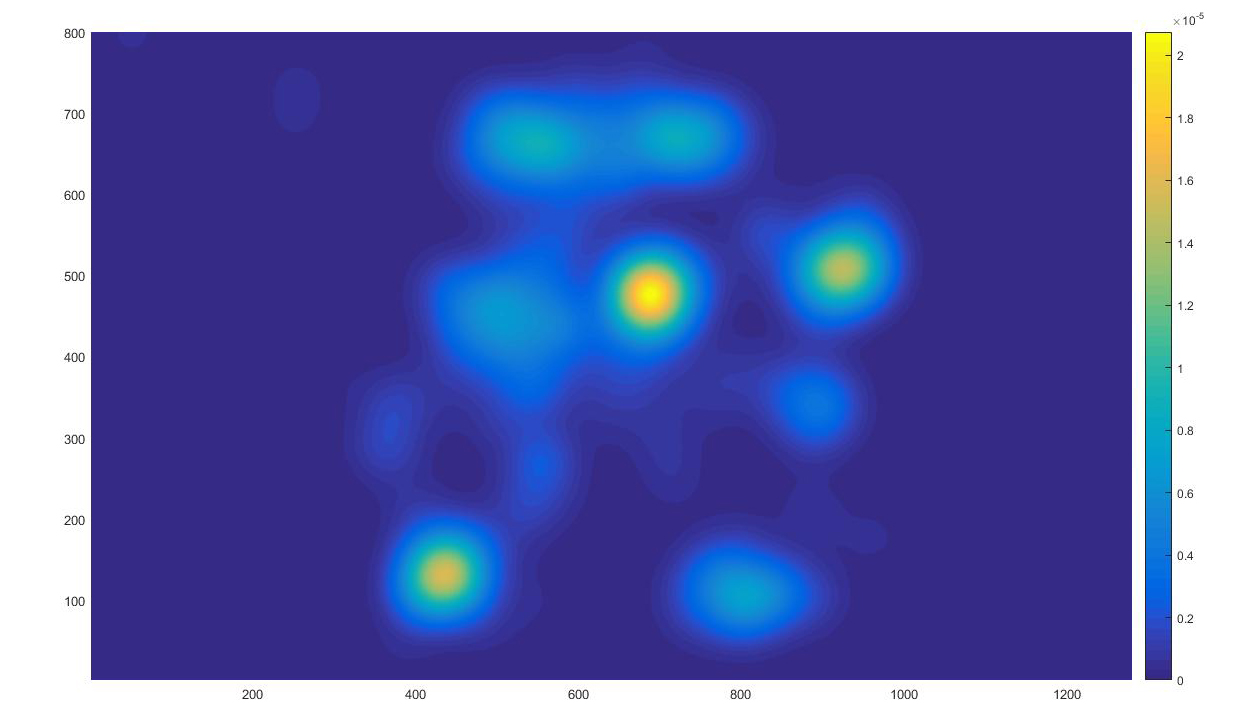
\includegraphics [width=\columnwidth]{fig/fig_eg_hm.jpg}
  \caption{图\ref{fig:aoi}中的例图的眼动热图。它是对眼睛在画面上的注视位置的概率分布的一种逼近或估计。}
  \label{fig:hm}
\end{figure}

考察代表眼动注视的位置的二维随机变量$(X, Y)$,则它的概率空间就是屏幕的分辨率空间(即把屏幕上的每一个像素认为是注视的一种可能的位置选择)。基于作用在该随机变量上的概率分布$P(X, Y)$,可以如下定义熵:

$$H(P)~=-\sum_{i=1}^{1280} \sum_{j=1}^{800} P(x_i, y_j)log_2(P(x_i, y_j))$$
其中: $$\sum_{i=1}^{1280}\sum_{i=1}^{800}~P(x_i, y_j)~=~1$$

而$(X, Y)$的概率分布$P(X, Y)$,实际上就是眼动热图,可以通过眼动数据进行估计。
热图的这种熵可以反映被试的眼动在空间上的分布的一致性或者凝聚度:当所有的注视聚焦在同一个像素上时,产生最小的熵值、让所有的注视平均地分散在屏幕上时,产生最大的熵值。
通过引入高斯核对每个注视点在空间上进行模糊处理,可以实现用少量的眼动采样据来估计注视在屏幕上的空间分布。
对一个屏幕横坐标位置为$x_0$,纵坐标位置为$y_0$,持续时长为$d$的眼动注视,它产生的高斯核可以表达为

$$d\cdot e^{-\frac{(x-x_0)^2 + (y-y_0)^2}{2\sigma^2}}$$

其中$\sigma$是高斯核的标准差。注意到上述的表达式并非标准的归一化的正态分布表达式,因为最终通过这些高斯核叠加得到的分布$P(X, Y)$还要进行归一化处理,以满足$\sum\sum P(X, Y) = 1$
除了用有限数据估计概率分布的需要之外,引入高斯核叠加的合理性还体现在人眼的注视事实上是与人眼的黄斑对应的具有一定半径的圆形范围,而实际的眼动注视也并非绝对固定不动而是包含一些微动行为的【】。另外考虑到眼动仪的检测本身具有一定的误差范围,高斯叠加的做法也令指标对误差具有一定的容忍度。\ref{fig:hm}展示了$\sigma=30px$时的热图的形态。
通过对40张实验页面的热图的熵的计算,发现其与美感评分表现出显著的负相关性($r = -0.5412, ANOVA F = 15.79 P = 0.0003$)。

\begin{table}[H]
\centering
\begin{tabular}{lrrrrr}
  \hline
  Source&SS&df&MS&F&Prob$>$F\\ \hline
  Groups&1.15861&1&1.15861&15.79&0.0003\\
  Error&2.78901&38&0.07339&&\\
  Total&3.94762&39&&&\\
  \hline
\end{tabular}
\caption{热图熵(视觉注意熵)的方差分析。}
\label{tab:ANOVA-vae-dw}
\end{table}

到目前为止,基于热图的熵是与美感表现出最强相关性的指标。鉴于热图有时会被认为是视觉注意的分布图,我们把上述定义的基于热图的熵称作视觉注意熵(Visual Attention Entropy,VAE)。


\subsection{相对VAE}
对于上面得到的VAE指标,存在着一定的理论缺陷。视觉注意熵与美感评分是负相关的,然而一个绝对低的VAE值并不意味着一个相当高的美感评分:一个只拥有相当少的内容的页面可能会得到一个相当低的VAE值,反之一个铺满内容的页面可能有相当高的VAE值,但显然这并不意味着前者一定比后者好看。理论上,具有不同内容复杂度的页面之间是无法通过VAE进行比较的。
为了解决该问题,我们引入了我们称之为相对VAE(relative, rVAE)的概念。为了让不同的页面的VAE可比较,需要首先考察他们各自的基础视觉注意熵(base VAE, bVAE)。对于一个页面,bVAE通过统计所有的被试各自的VAE的平均值得到,代表着一个无噪声扰动的VAE情况,是该页面的必要视觉注意成本。

$$bVAE~=~\frac{1}{n}\sum_{i=1}^n VAE(P_i)$$

其中n是被试人数,$VAE(P_i)$表示第i个被试的个体眼动注意熵。以bVAE作为一个先决条件,可以定义如下的相对视觉注意熵rVAE:

\begin{equation}
rVAE = \frac{VAE}{bVAE}
\label{formula:rvae}
\end{equation}

与VAE相比,rVAE与美感评分的关联性有显著提高,线性相关系数从-0.54提高到了-0.66。$ANOVA F = 26.84 P = 0.000008$。

\begin{table}[H]
\centering
\begin{tabular}{lrrrrr}
  \hline
  Source&SS&df&MS&F&Prob$>$F\\ \hline
  Groups&0.00336&1&0.00336&26.84&7.53E-06\\
  Error&0.00475&38&0.00013&&\\
  Total&0.00811&39&&&\\
  \hline
\end{tabular}
\caption{相对视觉注意熵(rVAE)的方差分析}
\label{tab:ANOVA-rvae-dw}
\end{table}

\ref{formula:rvae}似乎表明,基础视觉注意熵(bVAE)越大则相对视觉注意熵(rVAE)越小,则对应的美感有越大可能更好。但事实上,这不完全正确,由于之间的显著的相关性($r = 0.77$)表\ref{tab:corr},拥有较高的bVAE的页面很可能也会有较高的VAE。如果把bVAE当做是---

\begin{table}[H]
\centering
\begin{tabular}{l|rrrrrr}
  \hline
        &美感评分&注视总数&VAE&bVAE&rVAE\\ \hline
  美感评分 &1&0.33&\bfseries{-0.54}&-0.13&\bfseries{-0.66}\\
  注视总数&-&1&0.14&\bfseries{0.61}&-0.14\\
  VAE&-&-&1&\bfseries{0.77}&\bfseries{0.94}\\
  bVAE&-&-&-&1&0.52\\
  rVAE&-&-&-&-&1\\
  \hline
\end{tabular}
\caption{主要的眼动指标和美感得分两两之间的相关系数。}
\label{tab:corr}
\end{table}

上述关键指标间的相关性分析表明,bVAE与美感评分几乎没有相关性,但与注视的个数有较为显著的相关性。图\ref{fig:bvae}列出了所有的页面的个体VAE的盒图。

\begin{figure}[H]
  \centering
  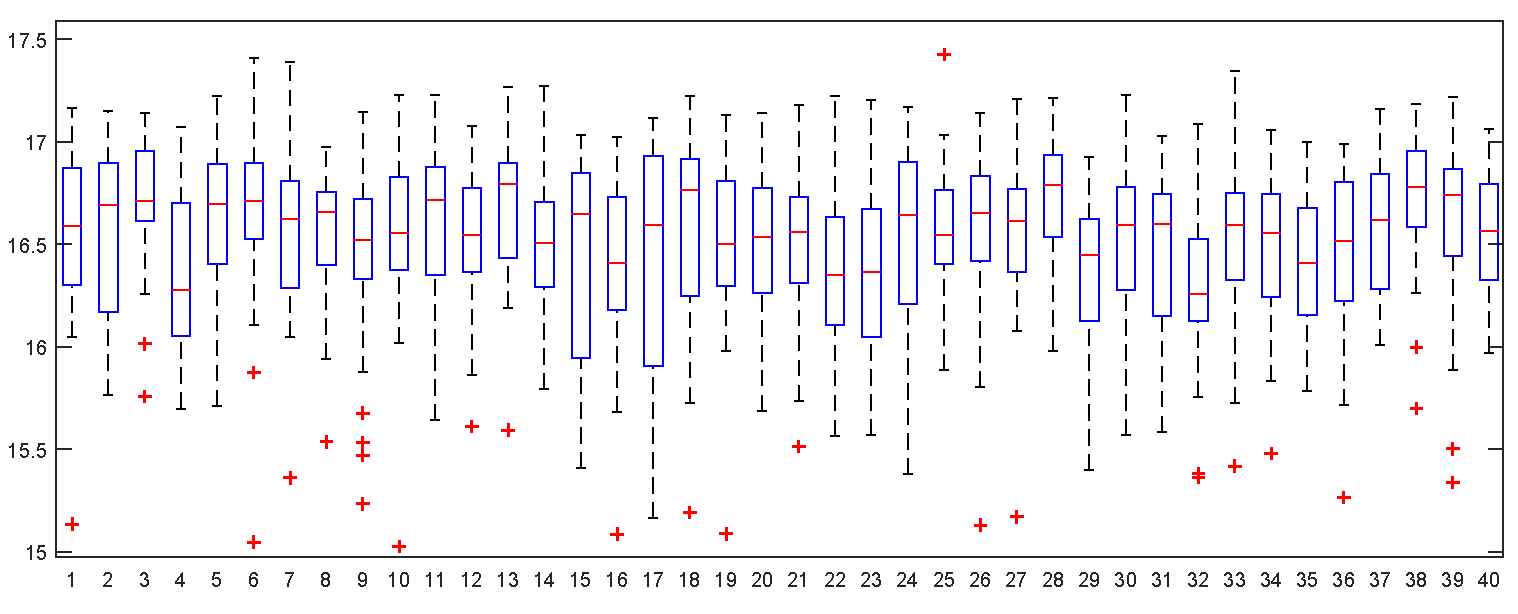
\includegraphics [width=1\columnwidth]{fig/fig_bvae.pdf}
  \caption{40张页面上30个被试的视觉重点熵(VAE)的盒图。页面从做到右按照美感评分排序。红色短横线代表均值,及该页面的基础视觉注意熵(bVAE)。在好坏页面见没有表现出显著差异。}
  \label{fig:bvae}
\end{figure}

bVAE的引入使得具有不同内容复杂度的页面的VAE变得可比较,并提供了对他们的美感评分的更为精确的预测。
图\ref{fig:box}展示了VAE和rVAE的方差分析盒图。展示了所有40张实验页面的美感评分分别关于VAE和rVAE的散点图。相比VAE,rVAE在区分好坏页面上具有更好的表现。

\begin{figure}[H]
  \centering
  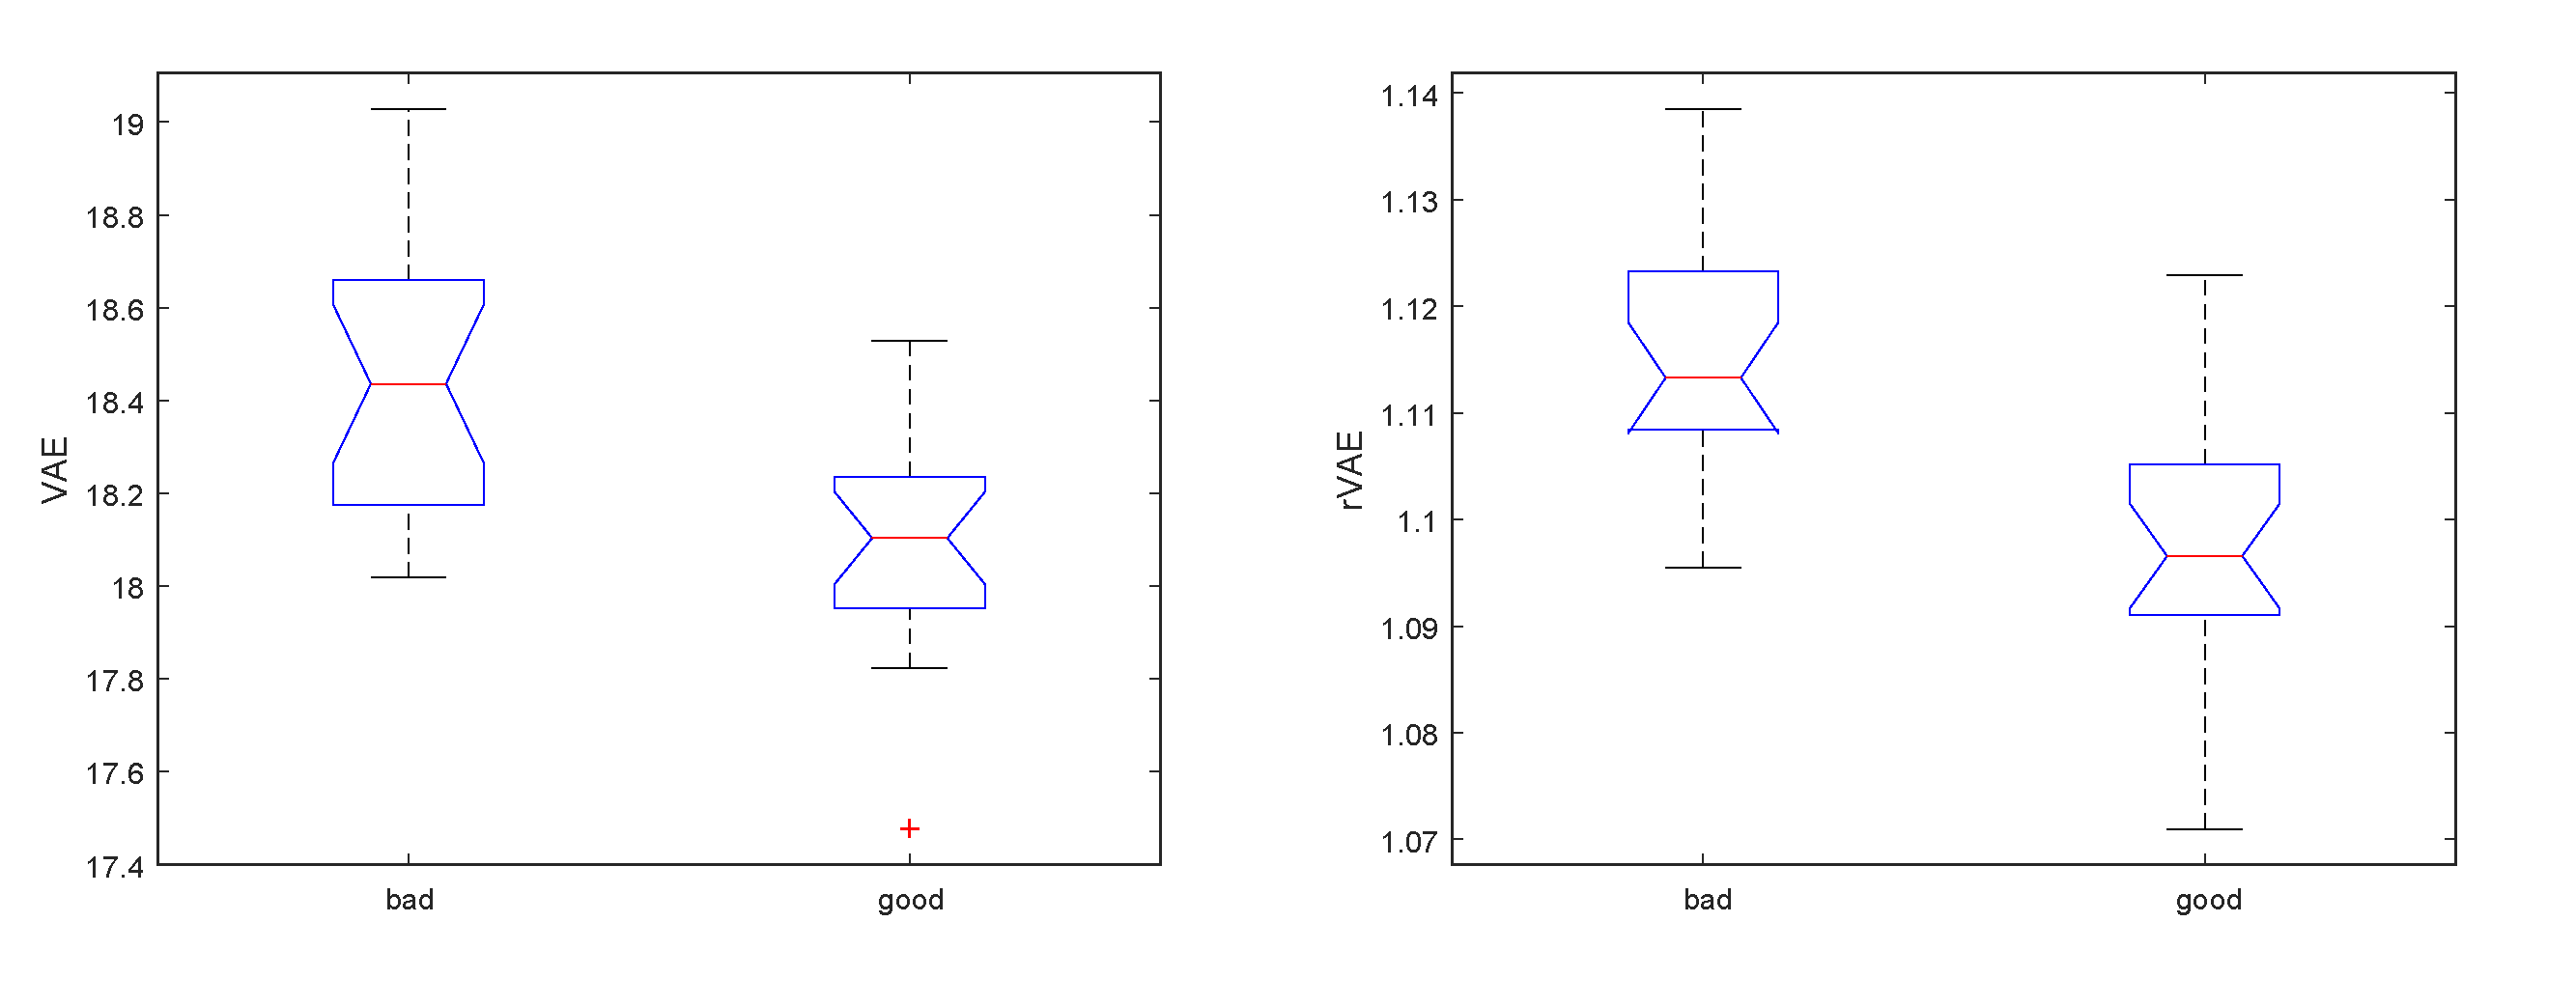
\includegraphics [width=1\columnwidth]{fig/fig_box.pdf}
  \caption{VAE和rVAE的盒图。左为VAE右为rVAE。显然,rVAE更显著地区分了好坏两个页面组别。}
  \label{fig:box}
\end{figure}

\begin{figure}[H]
  \centering
  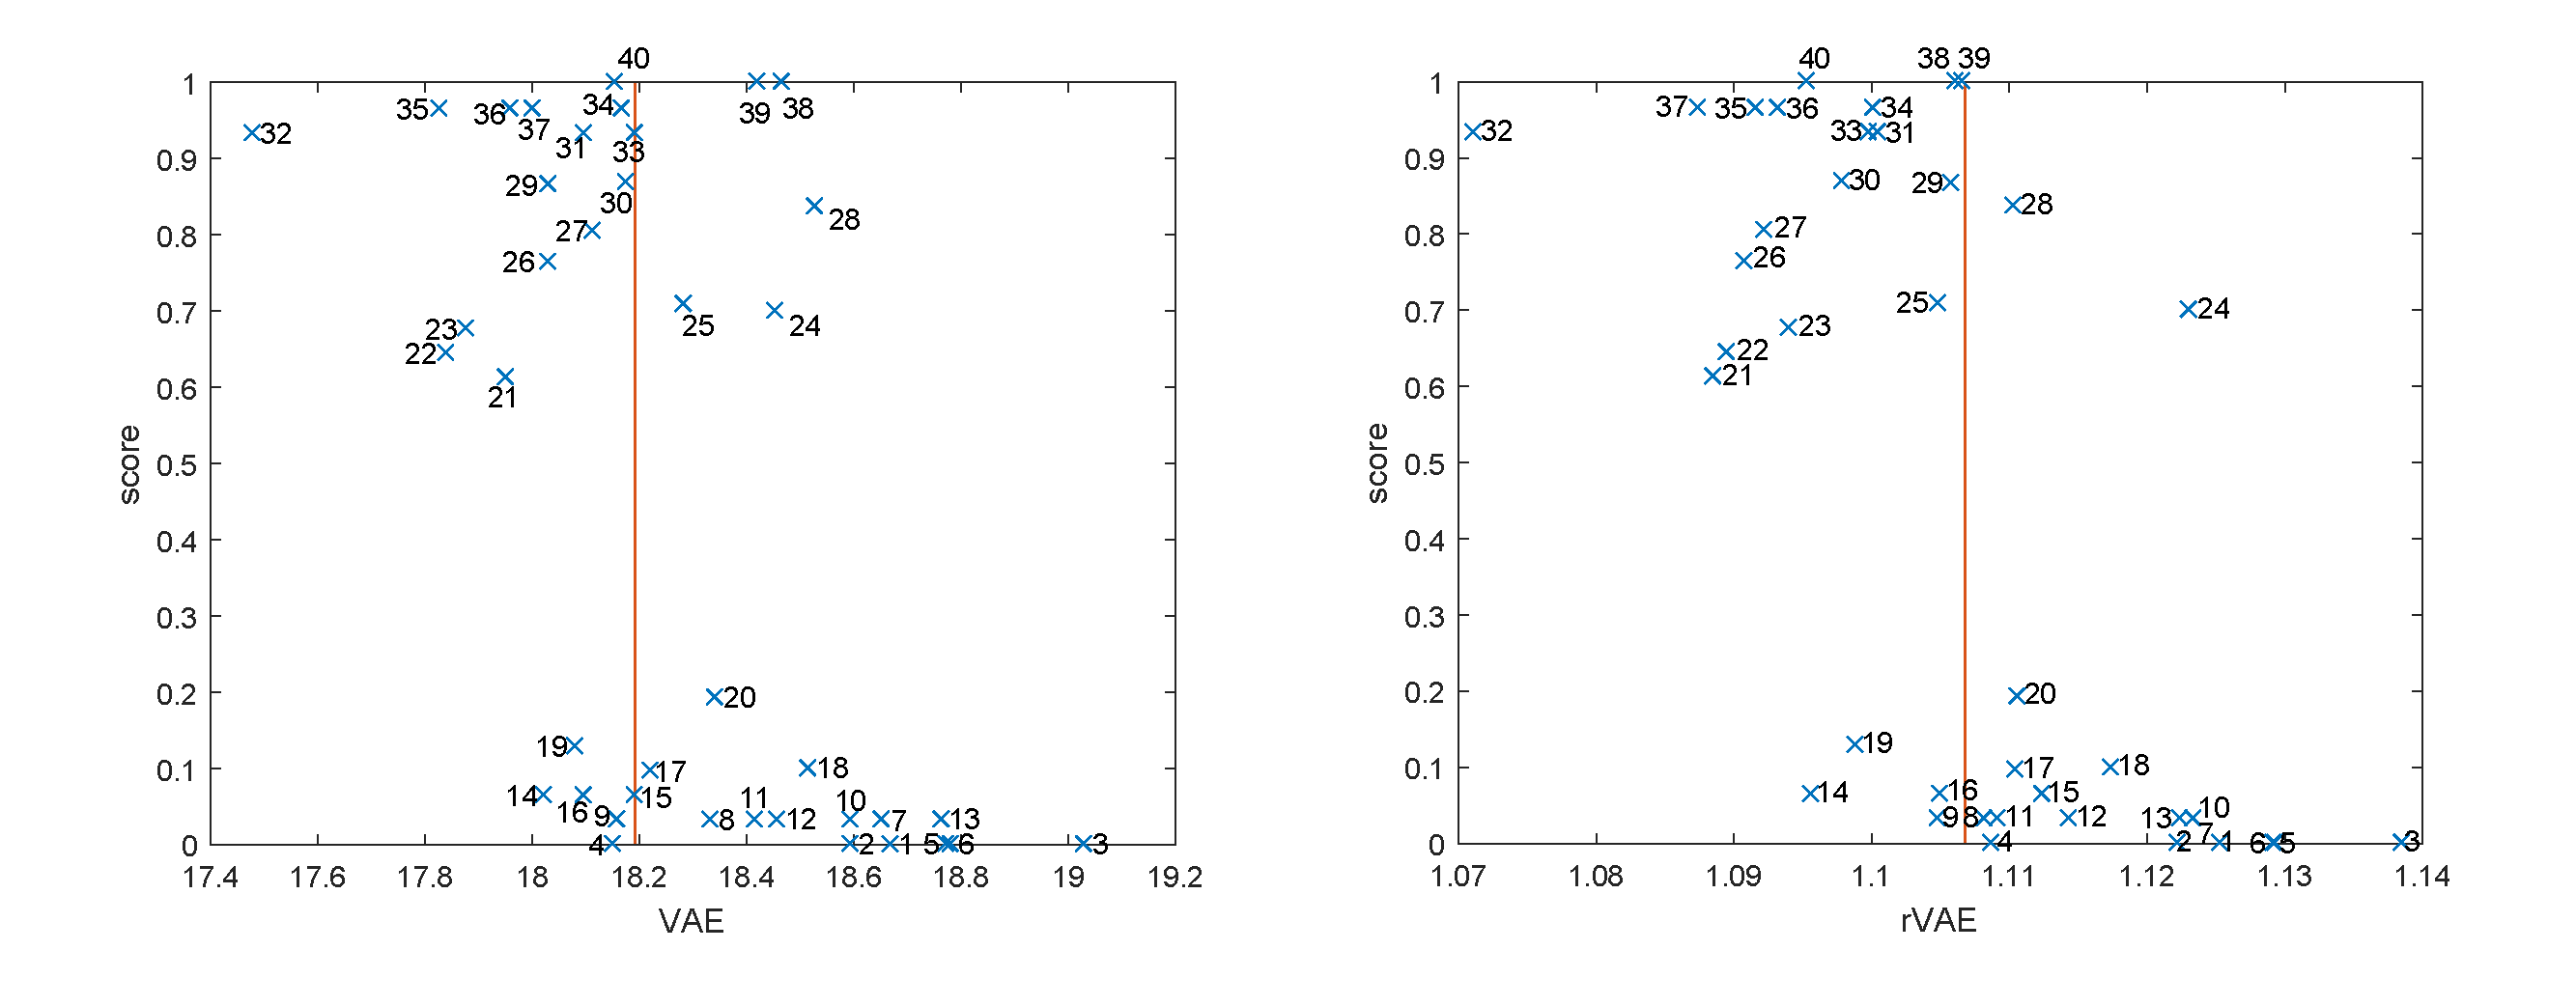
\includegraphics [width=1\columnwidth]{fig/fig_with-score.pdf}
  \caption{40张页面的VAE-得分散点图(左)和rVAE-得分散点图(右)。右图的点云更强的方向性。}
  \label{fig:with-score}
\end{figure}

\section{例外}
比较图\ref{fig:out}中的两张散点图我们发现总体而言相比VAE,rVAE使得好坏两组页面分得更开了,然而仍有一些被勿分类的页面。一个标注为24号的页面从整体的趋势中明显脱离,它有不错的美感评分,却在VAE和rVAE上都比较高。

\begin{figure}
  \centering
  
\includegraphics [width=\columnwidth]{fig/fig_outlier.jpg}
  \caption{例外图。左侧是例外的页面,图\ref{fig:with-score}中标号24的。如果全屏显示,你会觉得视觉上有一些决策压力。 右侧是略微改进后的版本,一些局部的视觉重点被调整了,从而视觉压力略微降低。}
  \label{fig:out}
\end{figure}

图\ref{fig:out}左面给出了这张页面的原始样本,不得不承认这张页面看起来还是不错的,包含了很多富有吸引力的因素如:漂亮的图片、色彩、平衡的布局等等。然而从一个设计师的角度,它还有不小的提升空间。全屏来看这张页面时,眼睛会感到一定的选择压力。这可能是因为视觉外围的一些密集的高对比造成的。图\ref{fig:out}的右面给出了这张页面经过细微版式调整后的版本。它阐明了细微的细节改动是如何改变给人的第一印象的。VAE本质上是受画面的边缘对比、复杂度等底层低级特征影响的,因而我们相信它能够表现观察者的视觉不适。可以肯定的是,我们通过VAE进行度量的视觉注意的流畅性美感判断具有不小的影响力。当然它也并非美感的全部。

\section{VAE的稳定性}
为了优化VAE的表现,我们分别考察熵与美感的相关性随着实验时间、纳入计算的被试人数以及热图高斯核的标准差的变化。
对给定的时刻t,我们统计发生在0-t时间段的眼动注视,并基于此计算VAE和rVAE,由此得到VAE和rVAE分别关于时间的变化的曲线。所有的曲线在开始时都表现出了较大幅的波动,然后逐步趋于稳定和平缓。图\ref{fig:with-t} 表现了实验页面的VAE随时间增大,rVAE随时间减小的趋势。
蓝色的曲线代表美感评价好的网页而红色的曲线代表美感评价坏的网页。显然好的页面随时间持续地有更小的VAE和rVAE值。此外在最后的时刻好坏的两个类别分的更开了。

\begin{figure}[H]
  \centering
  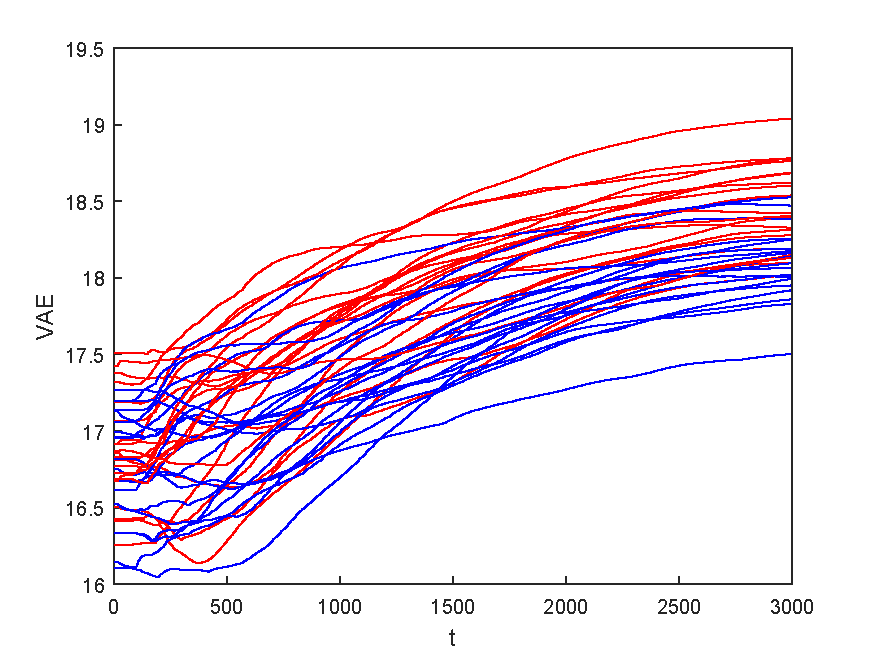
\includegraphics [width=0.85\columnwidth]{fig/fig_vae-t.pdf}
  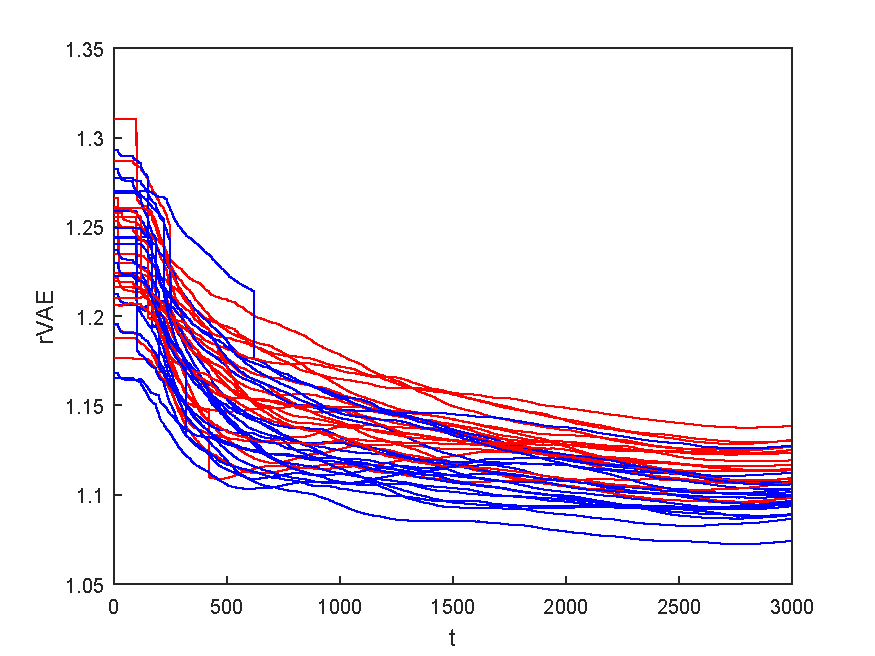
\includegraphics [width=0.85\columnwidth]{fig/fig_rvae-t.pdf}
  \caption{40张页面的VAE(上)和rVAE(下)随时间的变化图。蓝色曲线代表美感评分较好的网页组别,红色代表坏的。这些曲线随时间逐步趋于稳定,好的页面普遍给出了更小的VAE和rVAE值。两个组别随时间愈发分离。}
  \label{fig:with-t}
\end{figure}

图\ref{fig:corr-t}展现了熵和美感评分的相关系数随时间变化的曲线,在三秒的时刻相关系数取得了极值。由于我们没有记录3秒后的眼动数据,故没有办法看到后续的发展趋势。以母线的增长趋势,我们猜测相关系数可以变得更强。

\begin{figure}[H]
  \centering
  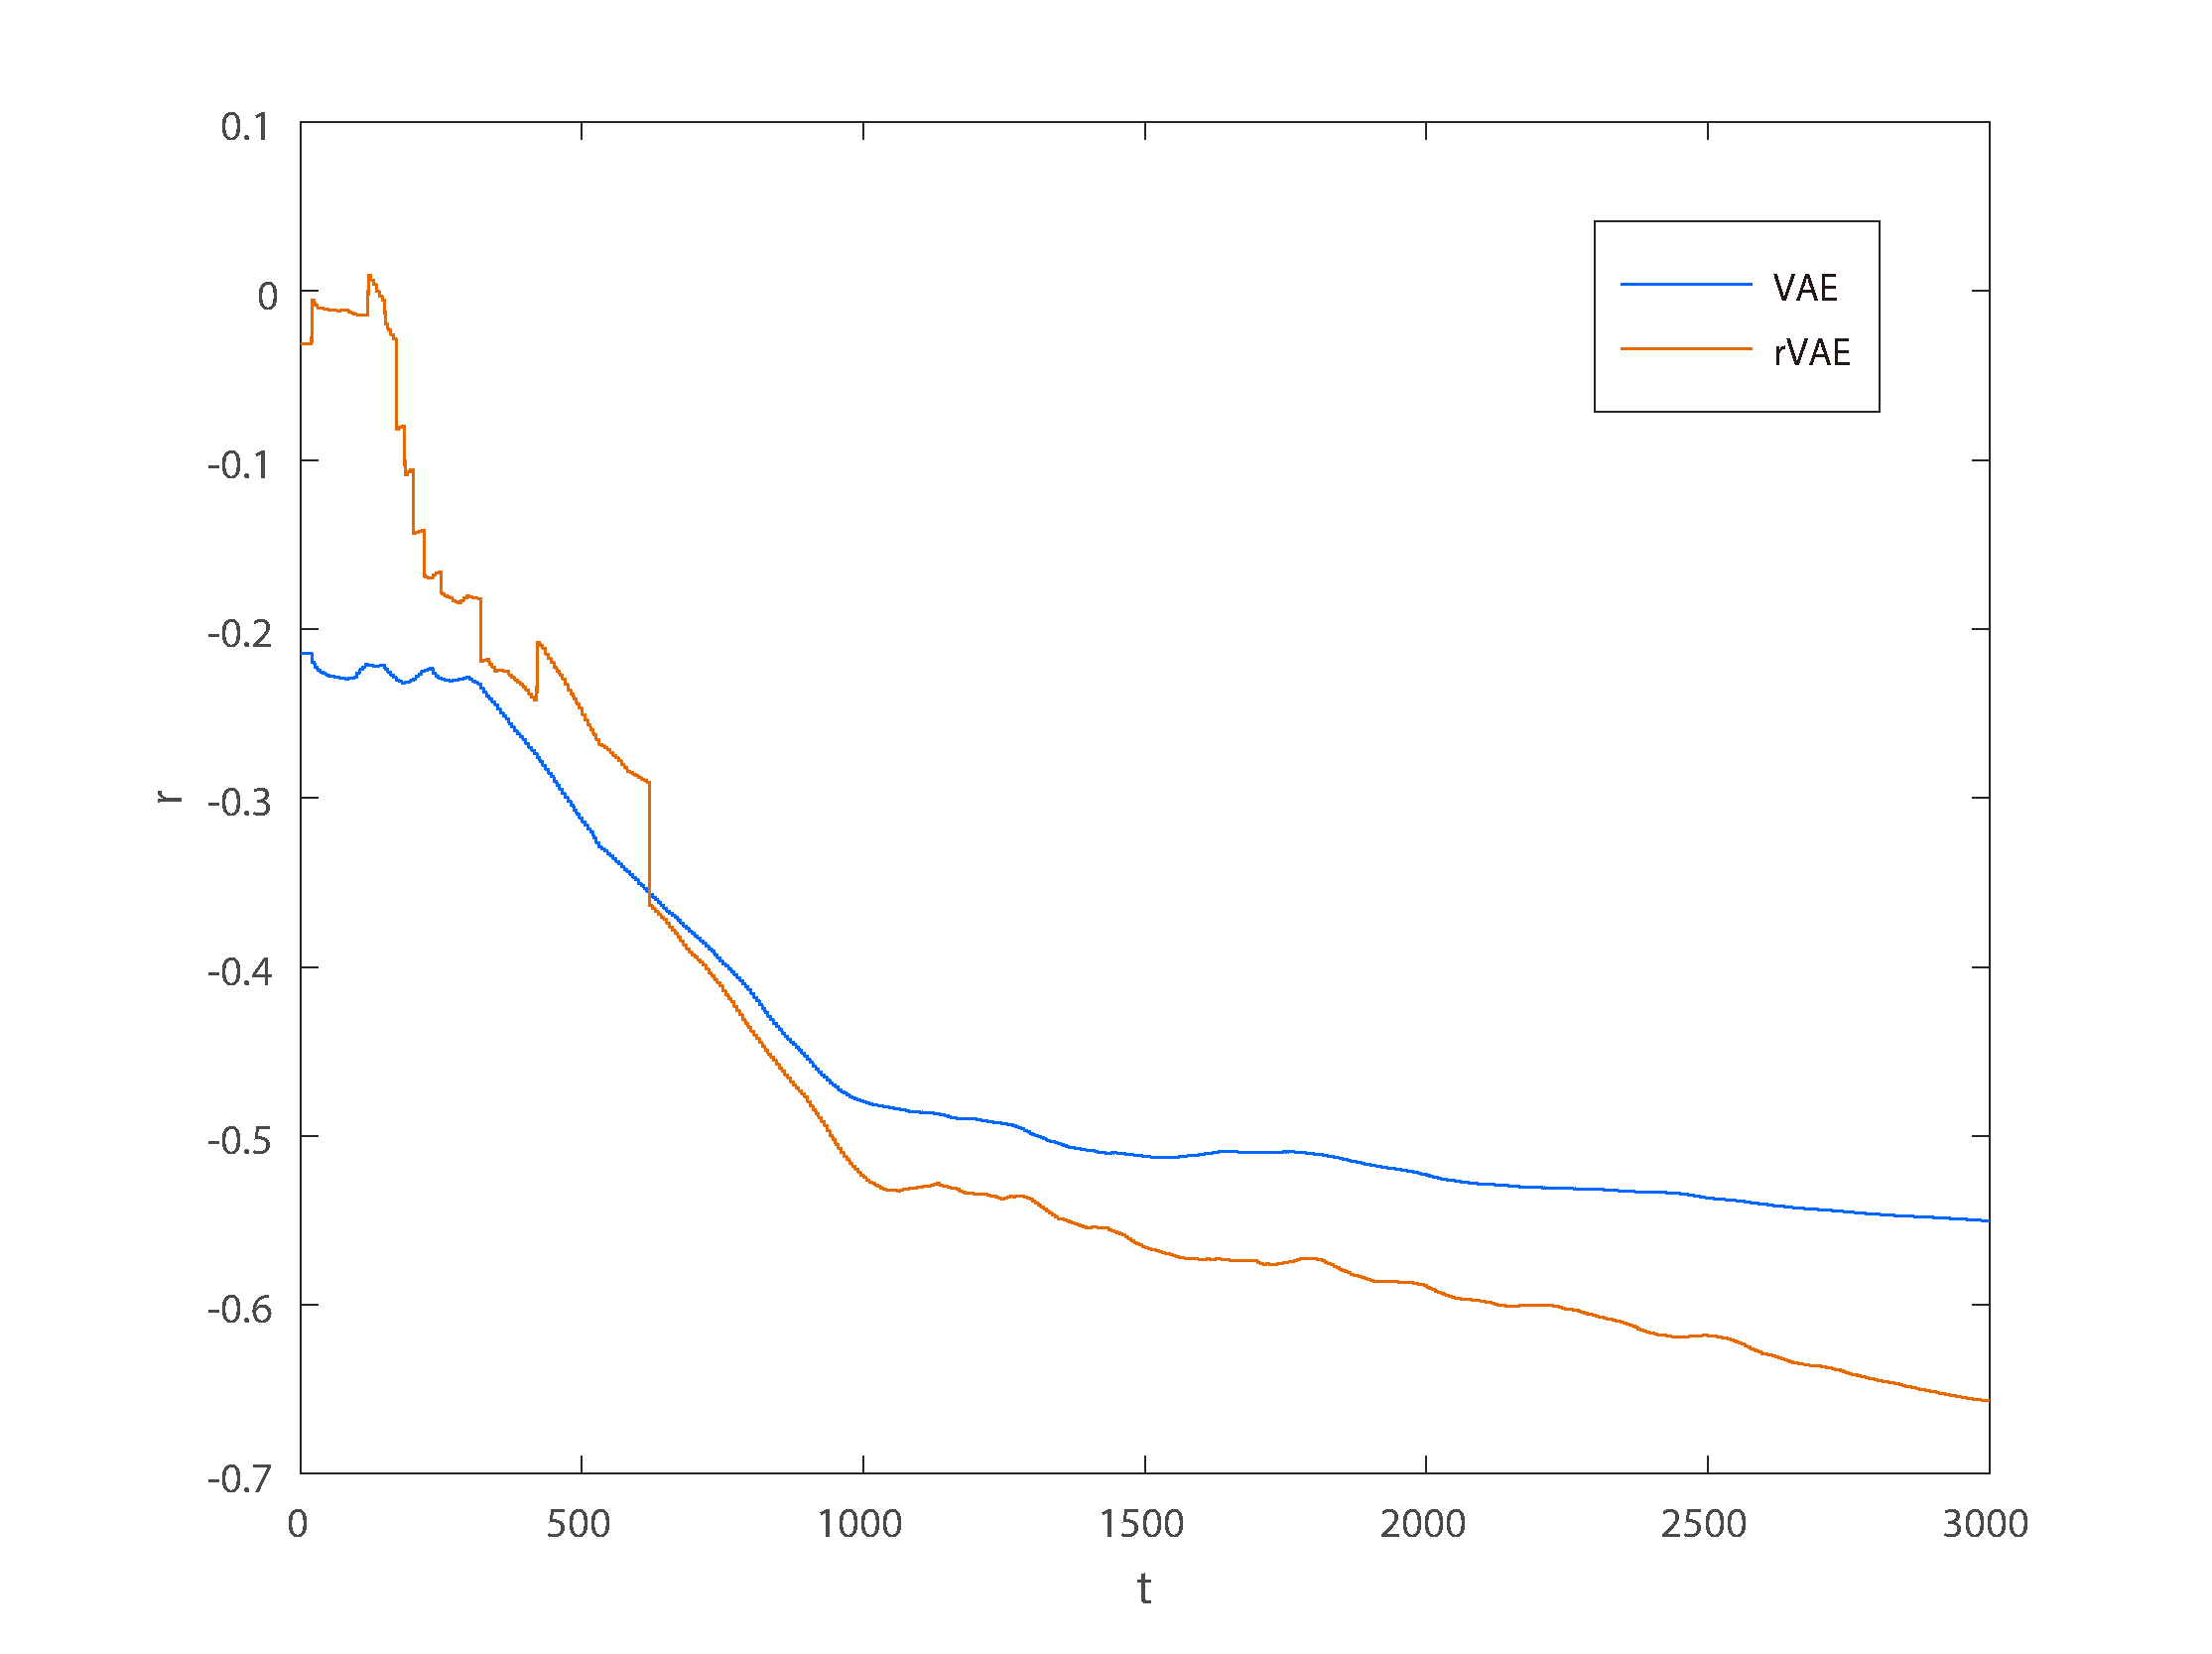
\includegraphics [width=0.85\columnwidth]{fig/fig_corr_t.pdf}
  \caption{两种视觉注意熵和美感评分的相关系数随时间的变化曲线。熵的显著性随时间愈发加强。1000ms开始rVAE的曲线稳定保持在VAE曲线的下方。依照发展的趋势,如果继续延长实验时间至超过3000ms,熵的表现可能更佳。}
  \label{fig:corr-t}
\end{figure}

图\ref{fig:with-user}展现了熵与美感评分的相关性随着被纳入计算的被试人数的增长而逐渐趋于稳定的趋势。图中的曲线结果是通过每次纳入一名随机被试的眼动数据获得的。似乎更多的被试人数会获得更好的与美感评分的关联性,但同时也以为着更高的时间成本和实验开销。

\begin{figure}[H]
  \centering
  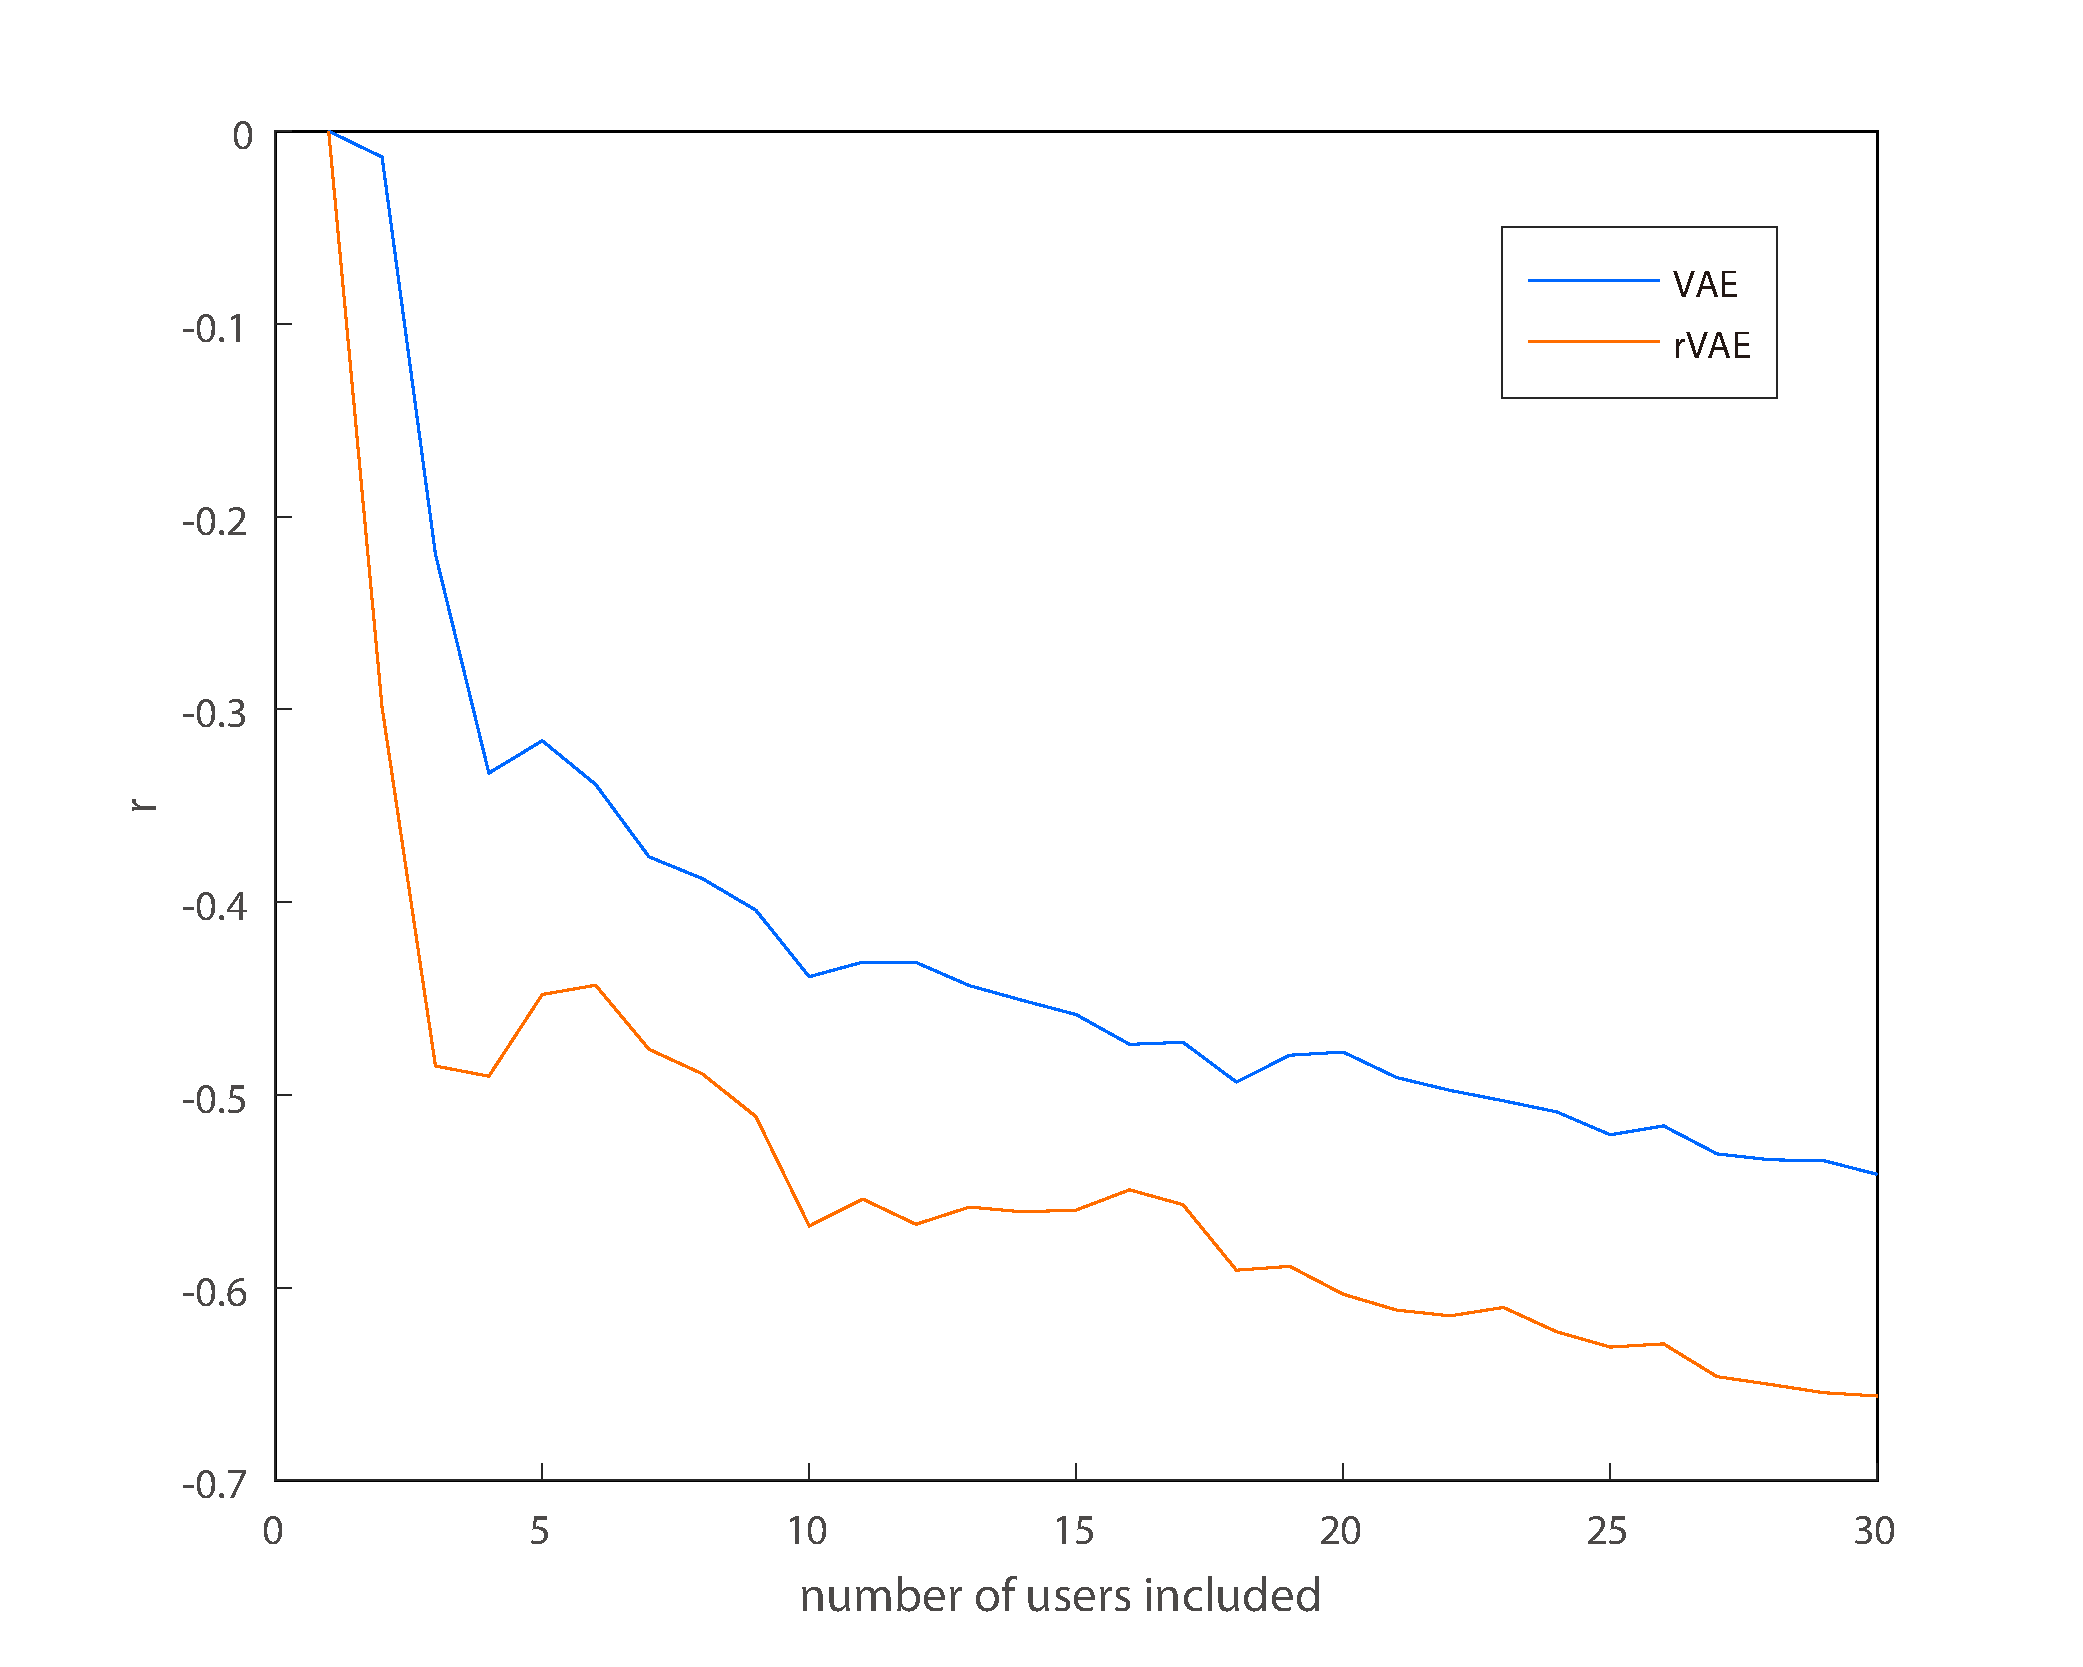
\includegraphics [width=0.85\columnwidth]{fig/fig_user.pdf}
  %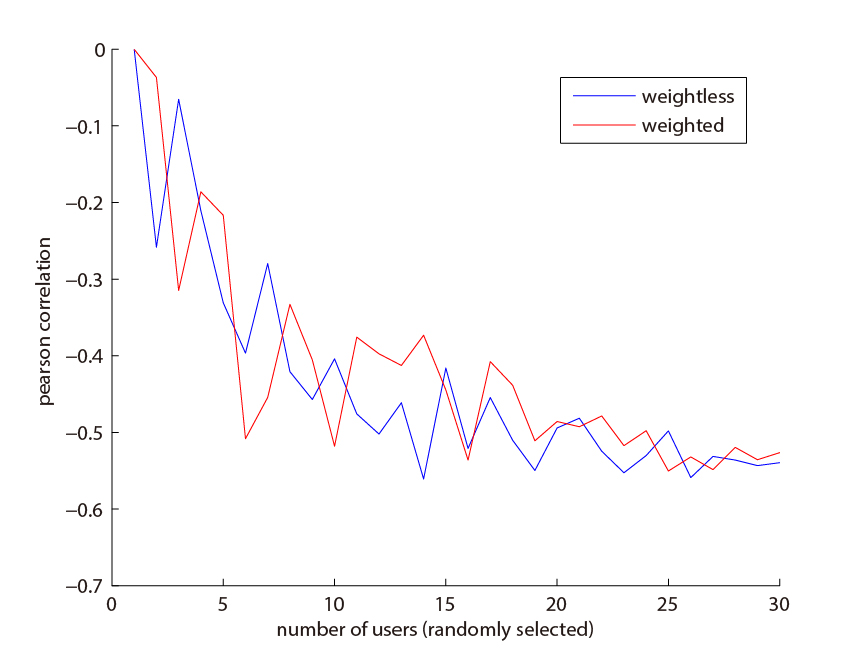
\includegraphics [width=80mm]{fig_vae_user.jpg}
  \caption{the correlations between the entropies and the aesthetic scores become more significant with the increasing numbers of subjects. The performance could be better if the number of subjects were larger than 30.}
  \label{fig:with-user}
\end{figure}

到目前为止我们的所有关于熵的计算都是基于热图高斯核$\sigma = 30$的基础上进行的。那么熵与美感的相关性对$\sigma$变化的敏感度如何呢?
\ref{fig:with-sigma}展现了相关系数随高斯核的平滑变化。在相当大的一个$\sigma$取值区间内,VAE和rVAE的表现都很稳定。VAE在$13px-60px$的区间内都有低于-0.5的与美感评分的相关系数;rVAE在$10px-120px$的区间内都有低于-0.6的与美感的相关系数。故熵的表现对于$\sigma$的取值是不敏感的。

\begin{figure}[H]
  \centering
  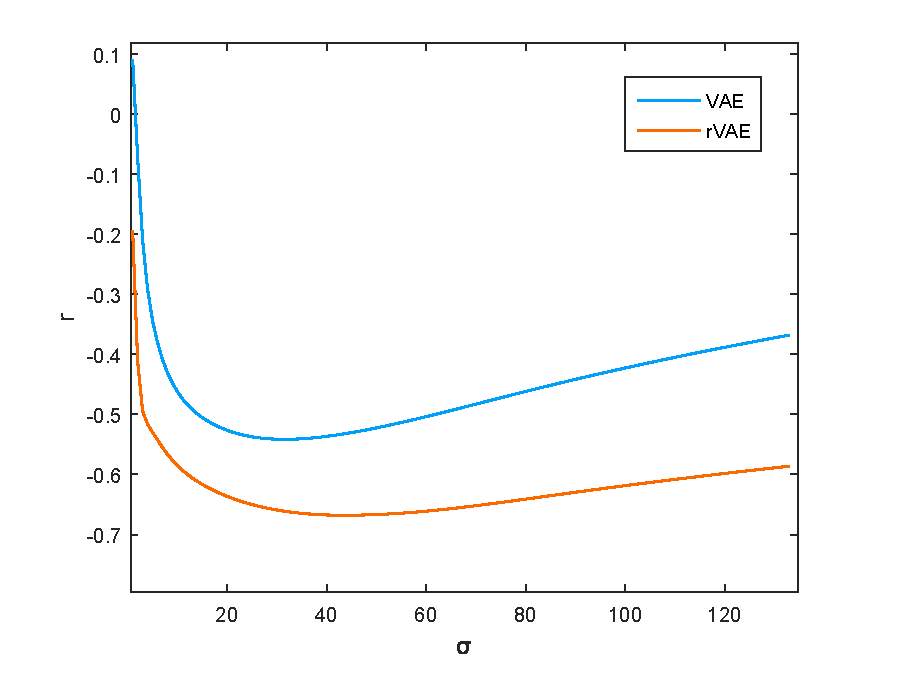
\includegraphics [width=0.85\columnwidth]{fig/fig_sigma.pdf}
  \caption{两种视觉注意熵与美感的相关性随热图高斯核标准差的变化的曲线图。曲线较为平滑,在很长一段区间内都保持在各自的极值附近:对VAE,从$20px$到$60px$都保持在-0.5以下,对rVAE,从$10px$到$120px$都保持在-0.6以下并在$40px$左右取得其极值。}
  \label{fig:with-sigma}
\end{figure}

上述的分析证实了VAE和rVAE在对美感的推测力方面的稳定性。并且看来,通过加长实验时间、扩大被试的规模和选择合适的$\sigma$取值,它们的表现还可以更好。

\section{讨论与小结}
实验证实了人的美感判断与眼动行为的确存在着联系。对注视序列和热图两个维度的香农熵的探索尝试表明,基于热图的视觉注意熵VAE对美感具有一定的推测里而基于马尔科夫假设的注视序列的熵则没有。VAE,视觉注意熵,可以解释成在分配有限的注意力资源时的混乱度。而他的改进版指标,rVAE,相对视觉注意熵,与我们的感知的美感有显著的相关性($r = -0.65$)。仅仅这单个指标对页面的美感好坏就有相当程度的预测力
。
VAE的成功的一部分因素归功于通过高斯核进行的插值,认为眼动注视的分布是连续的。同时3秒内的所有注视都投影在单个平面上,令数据密度更高。而注视序列熵失败的也许可以归咎于其基于时间的统计方式导致的数据量的稀疏。此刻仍很难说它与人的美感判断是无关的。也许未来可以找到更适用的模型来解决这个问题。

一个较低的VAE可以解释人们在眼睛动向和搜索上更少的代价付出。实验中好的网页拥有更小的VAE的趋势支持了流畅理论【】的说法,并一定程度上解释了为什么“好看的就是好用的”【】。VAE是基于眼动注视中的特定信息的。作为一个新的客观的眼动数据量化指标,它显然不仅仅是美感的一种度量,自然中的VAE与我们的观察和驾驶能力更相关。视觉注视在功能性上与鼠标指向很相似,这在一定程度上解释了为什么一些视觉引导相关的设计原则与Fitts规则(选择层级代价经验公式)很相似。

rVAE可以被理解成在屏幕范围的限制下用尽可能小的视觉注意代价(即VAE)去获取尽可能多的信息量(即bVAE)。这与基于进化论美学的“最大效益最小手段”的美学原则是一致的。进化论美学认为人类是为了提高生存和繁衍的成功率而进化出基础审美能力的。

眼动代表了显性和隐形注意的一种合作。虽然我们发现通过眼动行为来预测一个页面的美感至少需要约1000ms的眼动数据,我们对页面的第一印象的产生却只需要50-500ms【】。事实上,50ms仅仅足够完成一个对页面的快速“截屏”,我们的眼睛仍然停留在原地不动。这表明大脑可以通过50ms曝光的残留印象形成的隐形注意热图就作出美感的评价。
